\documentclass[fontset=windows]{article}
\usepackage[margin=1in]{geometry}
\usepackage{ctex}
\usepackage{setspace}
\usepackage{lipsum}
\usepackage{graphicx}
\usepackage{caption}
\usepackage{subcaption}
\usepackage[colorlinks=true,linkcolor=red]{hyperref}

\graphicspath{{figures/}}

\title{\heiti\zihao{2} Common-Source Stage with Degeneration}
\author{\songti zrrraa}
\date{2023.12.9}

\begin{document}
\maketitle
\thispagestyle{empty}

\section*{I/O Impedances of Deg. CS Stage}

Input Imp:

\begin{figure}[htbp]
    \centering
    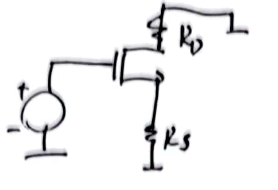
\includegraphics[scale=0.6]{1.jpg}
    \captionsetup{labelformat=empty}
    \caption{}
    \label{1}
\end{figure}

$R_{in}=\infty$ at low frequency. 

Output Imp $(\lambda>0)$ : 

\begin{figure}[htbp]
    \centering
    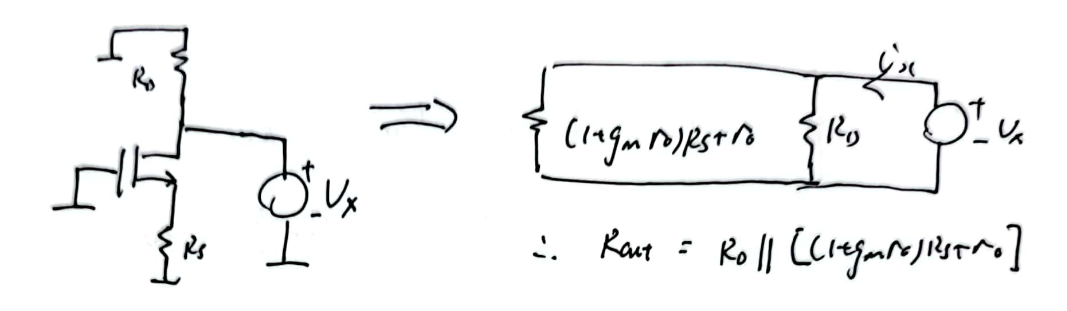
\includegraphics[scale=0.6]{2.jpg}
    \captionsetup{labelformat=empty}
    \caption{}
    \label{2}
\end{figure}

Borrow the output impedance formula of the degraded common source amplifier derived from the previous section, We can get: 

$$R_{out}=R_D||[(1+g_mr_o)R_s+r_o]$$

\section*{Biasing Techniques}

\begin{figure}[htbp]
    \centering
    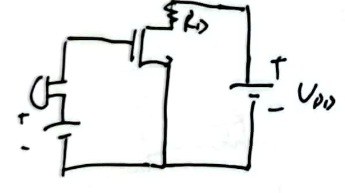
\includegraphics[scale=0.6]{3.jpg}
    \captionsetup{labelformat=empty}
    \caption{}
    \label{3}
\end{figure}

One possible way to bias the MOS is using resistors to divide the voltage. 

\begin{figure}[htbp]
    \centering
    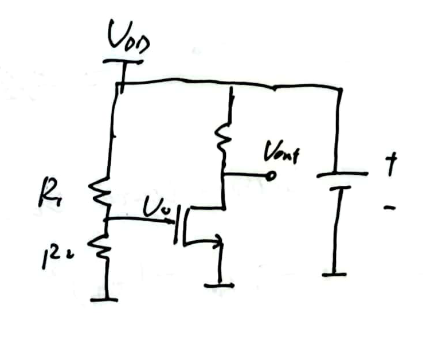
\includegraphics[scale=0.6]{4.jpg}
    \captionsetup{labelformat=empty}
    \caption{}
    \label{4}
\end{figure}

$$\frac{R_2}{R_1+R_2}V_{DD}=V_0$$

\section*{Observations $\lambda=0$}

\subsection*{Input Impedance = $R_1||R_2$}

\begin{figure}[htbp]
    \centering
    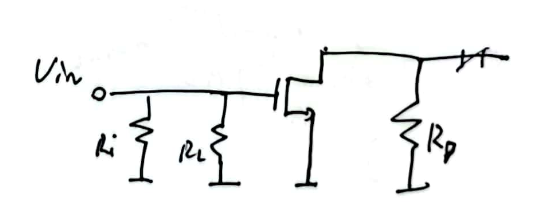
\includegraphics[scale=0.6]{5.jpg}
    \captionsetup{labelformat=empty}
    \caption{}
    \label{5}
\end{figure}

$$\frac{V_{out}}{V_{in}}=\frac{V_x}{V_{in}}*\frac{V_{out}}{V_x}=\frac{R_1||R_2}{R_1||R_2+R_{mike}}(-g_mR_D)$$

Choose $R_1||R_2>>R_{mike}$ to minimize the attenuation. 

\subsection*{Can we increase $R_D$ to increase gain?}

Of course, but make sure the MOSFET is in saturation zone. 

\subsection*{Sensitivity}

\begin{figure}[htbp]
    \centering
    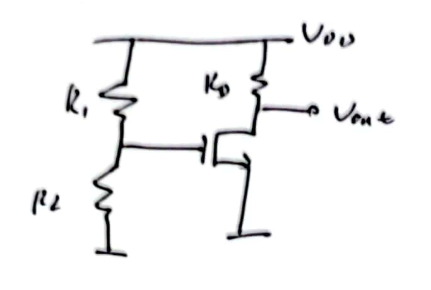
\includegraphics[scale=0.6]{6.jpg}
    \captionsetup{labelformat=empty}
    \caption{}
    \label{6}
\end{figure}

$$I_D=\frac{1}{2}\mu_nC_{ox}\frac{W}{L}(V_{DD}\frac{R_2}{R_1+R_2}-V_{TH})^2$$

$I_D$ is related to $V_{DD}$, $V_{TH}$, temp and the basic process parameters. 

\subsection*{Reduced Sensitivity with Deg. CS Stage}

\begin{figure}[htbp]
    \centering
    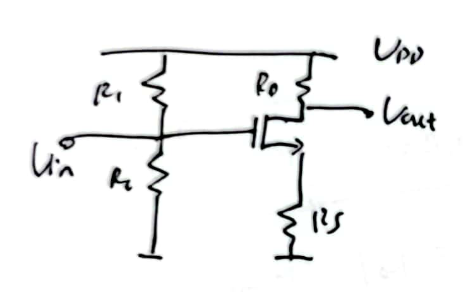
\includegraphics[scale=0.6]{7.jpg}
    \captionsetup{labelformat=empty}
    \caption{}
    \label{7}
\end{figure}

$$\frac{R_2}{R_2+R_1}V_{DD}=V_{GS}+I_DR_S$$

Part of the change in $V_{DD}$ will be shared by $R_S$, so $V_{GS}$ is more stable, I is more stable, and the gain is more stable.

\section*{Self-Biased CS Stage $\lambda=0$}

In this case, the drain voltage equals to the gate voltage, so the MOSFET always works in saturation zone. 

\begin{figure}[htbp]
    \centering
    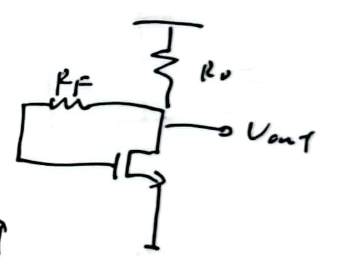
\includegraphics[scale=0.6]{8.jpg}
    \captionsetup{labelformat=empty}
    \caption{}
    \label{8}
\end{figure}

$$V_{DS}=V_{GS}=V_{DD}-I_DR_D$$

$$I_D=\frac{1}{2}\mu_nC_{ox}\frac{W}{L}(V_{DD}-I_DR_D-V_{TH})^2$$

Therefore, when $V_{TH}$ decreases, $I_D$ increases. 

\section*{Example}

\begin{figure}[htbp]
    \centering
    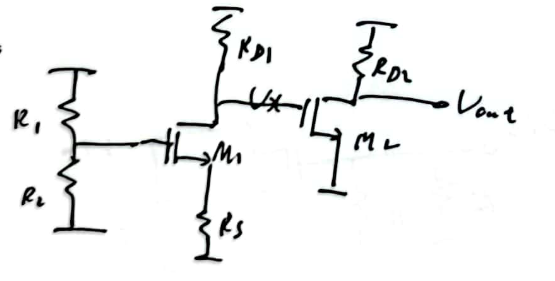
\includegraphics[scale=0.6]{9.jpg}
    \captionsetup{labelformat=empty}
    \caption{}
    \label{9}
\end{figure}

$$\frac{V_{out}}{V_{in}}=\frac{V_x}{V_in}*\frac{V_{out}}{V_x}=-\frac{R_{D1}}{\frac{1}{g_{m1}}+R_S}*(-g_{m2}*R_{D2})$$

This is called a cascade amplifier. 

\section*{Common-Gate Topology}

\begin{figure}[htbp]
    \centering
    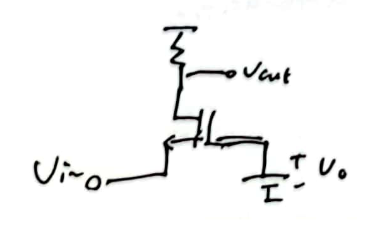
\includegraphics[scale=0.6]{10.jpg}
    \captionsetup{labelformat=empty}
    \caption{}
    \label{10}
\end{figure}

when $V_{in}$ increases, $V_{out}$ increases, so the gain is positive.  

\section*{Link}

\href{https://www.bilibili.com/video/BV1FD4y1R7Ah/?p=39}{Razavi Electronics Circuits 1: lectrue 39}
\end{document}